%!TEX root = ../thirdYearReport.tex
\appendix
\section{List of dissemination events}
%%%%%%%%%%%%%
%%%%%IIT%%%%%
%%%%%%%%%%%%%

\subsection{IIT contributions to dissemination}

4 invited talks, 4 organised international events, 6 talks at international conferences, 10 publications (2 journal, 7 internal conferences, 1 book chapter), 10 media coverage events, 11 iCub demos at dissemination events.

\subsubsection{Invited talks}

\begin{enumerate}
\item Invited speaker at the international workshop on Whole-Body Control for Robots in the Real World, held at the 2014 IEEE/RSJ international conference on intelligent robots and systems (IROS 2014). Contribution presented by Silvio Traversaro.
\item Invited speaker at the ?Cognitive Humanoid Robotics Research? workshop, held within the 2014 IEEE-RAS international conference on humanoid robots (Humanoids 2014). November 17th, 2014
\item Invited speaker at the Journées Nationales du GdR Robotique 2014, held at Grand amphithéâtre du Centre Arts et Métiers ParisTech, 151-155 boulevard de l'Hôpital, 75013 Paris. 30 October 2014.
\item Invited speaker at the first KoroiBot Summer School, held in Heidelberg from September 22nd to September 26th 2014. 
\end{enumerate}

\subsubsection{International events organisation}

Summary:
1) iCub Summer School
2) IROS 2015 event
3) Ballarò
4) Creative Mornings
5) RSS workshop
6) Festival della Scienza

-          CISCO conference Milano 26/1
-          CISCO conference Milano 28/1
-          Geo \& Geo Roma 25/2
-          Lancio cartone Transformers 1/3
-          ERF Vienna, workshop on humanoids in the laboratory (chimica, ecc.) 12/3
-          Conferenza stampa De Agostini (lancio X-makers) Barcellona 26/3
-          ITURO conference Istanbul, keynote 11/4
-          CSIFT Shanghai, investors presentation 22-24/4
-          Bal Robotov, invited forum on robotics, Mosca 29/4
-          Robobusiness, invited, Milan 30/4
-          Summer school on Sensing, Lille 21/5
-          Boston Woodshole, summer school CBMM, Robotics Afternoon, 18-22/8
-          Sky International, TV, 25/8
-          Uno Mattina, Rai1, 1/9
-          Rai Petrolio, 10/9
-          Expo, Padiglione Italia, 15/9
-          Aimeta conference, keynote, Genova, 16/9
-          Researchers night, invited, L’Aquila 26/9
-          Trieste Next Fest, invited, Trieste 27/9
-          IROS, Hamburg 28/9, 2/10
-          Caidate scientific talks, Caidate, 3/10
-          Space Challenge, keynote/lecture, Sofia, 6/10

\begin{enumerate}

\item The iCub Summer School, "Veni Vidi Vici", serves to consolidate and disseminate skills in software engineering for humanoid robots. Our goal is to foster collaboration on robot software across the boundaries and lifetimes of specific platforms and projects.
The school focuses on humanoid robotics and will host at least two iCub and a COMAN robot. Students will receive an initial training on the software infrastructure (middleware and tools) and will be required to work on a project of their choice. All participants are expected to be competent C/C++ programmers with an interest in working with others (and an agenda of their own). Info: \url{http://wiki.icub.org/wiki/VVV15}

\begin{figure}[!t]
	\begin{center}
		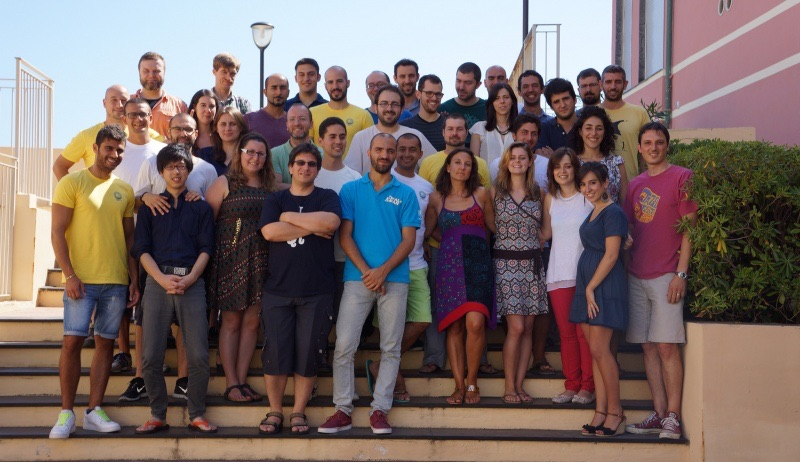
\includegraphics[height=4.5cm]{images/vvv.jpg}
		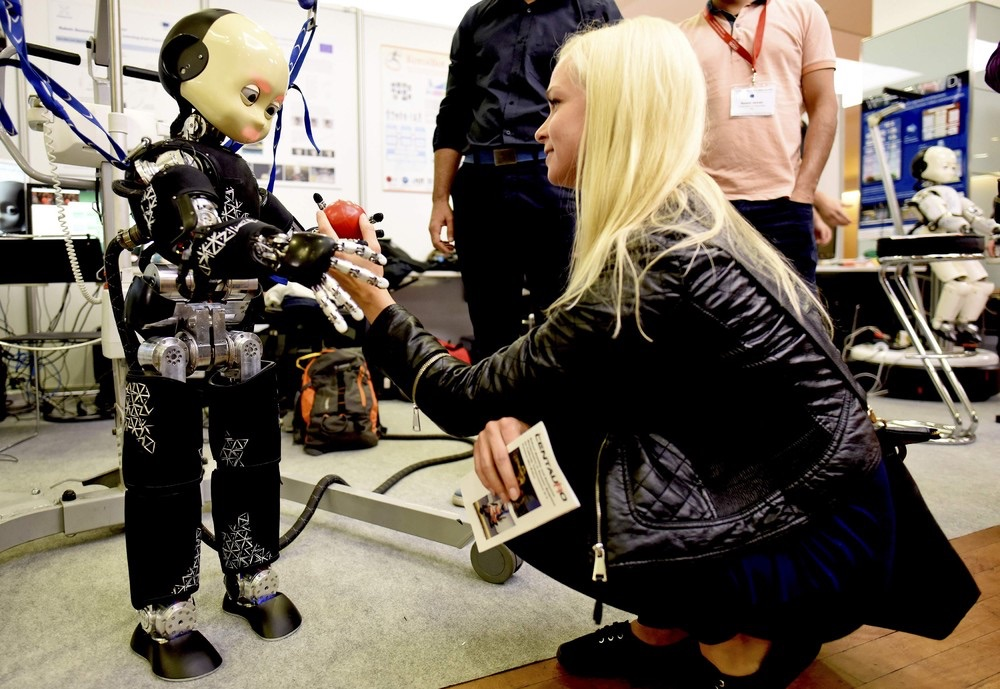
\includegraphics[height=4.5cm]{images/iros.jpg}
		\caption{Left: the iCub Veni-Vidi-Vici summer school. Right: the iCub at the IROS 2015 event organised by the robotics unit at the European Commission.}
		\label{fig:vvv}
	\end{center}
\end{figure}

\item During the IROS 2015 International Conference at Hamburg, different versions of iCub (the Genova Black, and the Heidelberg version) were shown in an exhibition. For three days, iCub interact with visiting people performing different demos, such as torque balancing and the red ball demo. Photo by Fabian Bimmer/Reuters)


\item iCub has been a special guest in Ballar\'o, an italian political show on the public television network.

\item In May, Francesco Nori was an invited speaker at the Creative Mornings event. The talk gave historical and philosophical motivations that guided recent research activities towards the problem of studying how humans interact with the environment and among themselves. The iCub was also presented, as an open-source platform capable of advancing the state-of-the-art in various directions, e.g. decisional autonomy, dependability/adaptability, perception and, in a single all-embracing word, cognitive abilities.

\item In July, during the RSS conference in Rome, a full day workshop titled ?Towards a Unifying Framework for Whole-body and Manipulation Control? has been organised. Topics covered the following areas:
\begin{itemize}
\item Contacts planning and control
\item Whole-body task control
\item Compliant whole-body movements
\item Dynamics in humanoid robots
\item Machine learning and optimization methods for contact planning and control
\end{itemize}

\item From 22nd of October to 1st of November 2015, the iCub will be showed at the ``Festival della Scienz''. Festival della Scienza, now at its 13th edition, is a publicly opened event which focus on science. During this festival, temporary laboratories and exhibition booths are prepared where researchers and scientists can show and explain to people their work. Presentations are targeted to different audiences, from children to university students to adults. This year festival theme is ?Equilibrium?, and iCub will perform daily showing balancing demos. 

\end{enumerate}

\subsubsection{Talks at international conferences}

\begin{enumerate}
\item Talk by Francesco Nori. A. Del Prete, F. Romano, L. Natale, G. Metta, G. Sandini and F. Nori. Prioritized Optimal Control. 2014 IEEE International Conference on International Conference on Robotics and Automation (ICRA 2014). 
\item Talk by Francesco Romano. Romano F., Fiorio L., Sandini G. and Nori F. 2014, ?Control of a two-DOF manipulator equipped with a pnr- Variable Stiffness Actuator?, 2014 IEEE Multi-Conference on Systems and Control, Antibes, France, October 8-10, 2014.
\item Talk by Luca Fiorio. Fiorio L., Romano F., Parmiggiani A., Sandini G. and Nori F. 2014, ?Stiction Compensation in Agonist-Antagonist Variable Stiffness Actuators?, 2014 Robotics: Science and Systems Conference, Berkeley, California, USA, July 12-16, 2014.
\item Talk by Serena Ivaldi. Ivaldi S., Peters J., Padois V. and Nori F. 2014, ?Tools for simulating humanoid robot dynamics: a survey based on user feedback?, Proceedings of the International Conference on Humanoid Robots (HUMANOIDS 2014)., Madrid, Spain, November 18-20, 2014, Spain.
\item Talk by Serena Ivaldi. Nori F., Peters J., Padois V., Babic J., Mistry M. and Ivaldi S. 2014, ?Whole-body motion in humans and humanoids?, Proceedings of the Workshop on New Research Frontiers for Intelligent Autonomous Systems (NRF-IAS).
\item Talk by Carlo Ciliberto. Ciliberto C., Fiorio L., Maggiali M., Natale L., Rosasco L., Metta G., Sandini G. and Nori F. 2014, ?Exploiting global force torque measurements for local compliance estimation in tactile arrays?, IEEE/RSJ International Conference on Intelligent Robots and Systems (IROS 2014), Chicago, USA, September 14-18, 2014.
\end{enumerate}


\subsubsection{Pubblications}

Del Prete A., Nori F., Metta G. and Natale L. 2015, ?Prioritized motion–force control of constrained fully-actuated robots: “Task Space Inverse Dynamics”?, Robotics and Autonomous Systems, vol. 63,no. 1, pp. 150?157.

F Nori, S Traversaro, E Jorhabib, F Romano and D Del Prete A.; Pucci. iCub Whole-body Control through Force Regulation on Rigid Noncoplanar Contacts. Frontiers in Robotics and AI.

H E Mingo, S Traversaro, R Alessio, F Mirko, A Settimi, F Romano, L Natale, A Bicchi, F Nori and G Tsagarakis. A Yarp based plugin for Gazebo Simulator. In Modelling and Simulation for Autonomous Systems. 2014

Ciliberto C., Fiorio L., Maggiali M., Natale L., Rosasco L., Metta G., Sandini G. and Nori F. 2014, ?Exploiting global force torque measurements for local compliance estimation in tactile arrays?, IEEE/RSJ International Conference on Intelligent Robots and Systems (IROS 2014), Chicago, USA, September 14-18, 2014.

Del Prete A., Romano F., Natale L., Metta G., Sandini G. and Nori F. 2014, ?Prioritized Optimal Control?, IEEE International Conference on Robotics and Automation (ICRA2014), IEEE, Hong Kong, China, May 31-June 7, 2014, 2014.

Del Prete A., Mansard N., Nori F., Metta G. and Natale L. 2014, ?Partial Force Control of Constrained Floating-Base Robots?, IEEE/RSJ International Conference on Intelligent Robots and Systems (IROS 2014), Chicago, Illinois, September 14–18, 2014.

Fiorio L., Romano F., Parmiggiani A., Sandini G. and Nori F. 2014, ?Stiction Compensation in Agonist-Antagonist Variable Stiffness Actuators?, 2014 Robotics: Science and Systems Conference, Berkeley, California, USA, July 12-16, 2014.

Ivaldi S., Peters J., Padois V. and Nori F. 2014, ?Tools for simulating humanoid robot dynamics: a survey based on user feedback?, Proceedings of the International Conference on Humanoid Robots (HUMANOIDS 2014)., Madrid, Spain, November 18-20, 2014, Spain.

Mingo H.E., Traversaro S., Alessio R., Mirko F., Settimi A., Romano F., Natale L., Bicchi A., Nori F. and Tsagarakis G. Nikos 2014, ?A Yarp based plugin for Gazebo Simulator?, 2014 Modelling and Simulation for Autonomous Systems,.

Nori F., Peters J., Padois V., Babic J., Mistry M. and Ivaldi S. 2014, ?Whole-body motion in humans and humanoids?, Proceedings of the Workshop on New Research Frontiers for Intelligent Autonomous Systems (NRF-IAS),.

Romano F., Fiorio L., Sandini G. and Nori F. 2014, ?Control of a two-DOF manipulator equipped with a pnr- Variable Stiffness Actuator?, 2014 IEEE Multi-Conference on Systems and Control, Antibes, France, October 8-10, 2014.

\subsubsection{Media coverage}

\begin{itemize}

\item \url{http://video.repubblica.it/edizione/genova/genova-icub-il-robot-bambino-ora-sta-in-piedi/167466/165953}

\item \url{http://www.nextme.it/tecnologia/robotica/8958-icub-robot-morbidi-8-anni-video}

\item \url{http://video2k.is/index.php/videos/v/jaTEbCsFp_M/yt}

\item \url{http://meta-guide.com/videography/100-best-icub-robot-videos/}

\item \url{http://www.33rdsquare.com/2015/02/icub-becomes-master-of-balancing.html}

\item \url{http://video.corriere.it/robot-icub-fa-progressi-equilibrio/a20154ce-c961-11e4-84dd-480351105d62}

\item \url{http://www.geniuslab.org/storie/con-il-raggiungimento-dellequilibrio-icub-accorcia-i-tempi-per-entrare-nelle-nostre-case/}

\item \url{http://www.rainews.it/dl/rainews/media/Occhi-grandi-e-sorrisone-il-cucciolo-robot-muove-i-primi-passi-93898c5e-032b-4f2f-9240-14ee1682e87c.html}

\item \url{https://www.youtube.com/watch?v=jtjBsBE5GIIandt=3m36s}

\item \url{http://www.rai.tv/dl/RaiTV/programmi/media/ContentItem-38aee841-5df8-48e2-ba54-064c0457bc45.html#p=0}
\end{itemize}

\subsubsection{iCub at international events}

\begin{enumerate}

\item Innovation Convention 2014 Brussels
\item European Robotics Forum Rovereto
\item Innorobo 2014 Lyon
\item World Science Festival New York City
\item Automatica 2014 Munich
\item Festival della Comunicazione Camogli
\item European Maker Faire Roma
\item RAI Studios [i Fatti Vostri] Roma
\item Humanoids 2014 Madrid
\item RAI Studios [Rai2Next] Roma
\item Embedded Technology 2014 Tokyo

\end{enumerate}

%%%%%%%%%%%%%
%%%%TUD%%%%%%
%%%%%%%%%%%%%
\subsection{TUD contributions to dissemination}

%TODO update
15 invited talks, 4 organised international events, 7 publications (7 internal conferences), 7 media coverage events


\subsubsection{Invited talks}

\begin{enumerate}
%year three (03.2015-02.2016)

% Roberto
\item 16 Oct 2015 University College London, London, UK, host: Guy Lever.
\item 14 Oct 2015 University of Oxford, Oxford, UK, host: Michael Osborne, Machine Learning Research Group.
\item 13 Oct 2015 Imperial College London, London, UK, host: Stefan Leutenegger, Dyson Robotics Lab.
\item 03 Jun 2015 University of British Columbia, Vancouver, Canada, host: Mark Schmidt.
\item 02 Jun 2015 University of Washington, Seattle, US, host: Dieter Fox, Robotics and State Estimation Lab.
\item 01 Apr 2015 TU Freiburg, Freiburg, Germany, host: Frank Hutter.

%Elmar
\item 11/2015 Understanding Human Motor Control through Robotics Applications. Invited Talk in Prof. Constantin Rothkopf’s seminar on ’research and applications of psychology in IT’, Darmstadt, Germany.
\item 02/2015 Probabilistic Inference and Modeling of Human Motor Skill Learning. Invited Talk. Workshop with Marc Toussaint’s group, Wolfram Burgard’s group and Oliver Brock’s group, Manigod, France.


%Jan
% \item 9/17/2014 IEEE/RSJ International Conference on Intelligent Robots and Systems (IROS), Session [1] Keynote for the Learning by Demonstration Session Topic, Chicago, USA
% \item 7/16/2014 13th International Conference on Intelligent Autonomous Systems (IAS-13), Padua, Italy 
% \item 7/11/2014 British Machine Vision Association (Vision for language and manipulation), London, UK
% \item 7/9/2014 IEEE/ASME Conference on Advanced Intelligent Mechatronics (AIM2014), Besancon, France
% \item 3/27/2015 RSS 2015 Symposium: Frontiers of Robotics, New Brunswick, USA 
% \item 9/14/2014 IROS Workshop: Machine Learning in Planning and Control of Robot Motion, Chicago, USA
% \item 6/5/2014 ICRA Workshop: iCub and Friends, Hong Kong, China
% \item 2/6/2015 Carnegie Mellon University, Robotics Institute Lecture Series , Host: S. Srinivasa, J.A. [55] Bagnell, Pittsburgh, PA, USA
% \item 1/16/2015 Technische Universität München, Host: E. Steinbach, Munich, Germany [56]
% \item 12/4/2014	KIT, Host: W. Juling, Karlsruhe, Germany [57]
% \item 11/28/2014	ETH Zürich, ETH Distinguished Lecture Series, Host: R. Siegwardt, Zürich, Switzerland
% \item 7/7/2014 Universität Hamburg, Host: U. von Luxburg, Hamburg, Germany [59]
% \item 5/9/2014 Université de Liege, Host: D. Ernst, Liege, Belgium [60]
% \item 2/5/2014 ABB AG, Corporate Research Center, Robotics and Manufacturing, Host: H. Ding, Ladenburg, Germany
% \item 2/4/2014 Technical University of Graz, Host: W. Maas, Graz,Austria [62]
\end{enumerate}


\subsubsection{Publications}

\begin{enumerate}
%year three (03.2015-02.2016)
%journals
\item E Rueckert, D Kappel, D Tanneberg, D Pecevski and J Peters. Recurrent Spiking Networks Solve Planning Tasks. Scientific Reports, Nature Publishing Group, 2016.
\item R Calandra, A Seyfarth, J Peters and M P Deisenroth. Bayesian optimization for learning gaits under uncertainty. Annals of Mathematics and Artificial Intelligence, pages 1–19, 2015.
%conferences
\item J Kohlschuetter, J Peters and E Rueckert. Learning Probabilistic Features from EMG Data for Predicting Knee Abnormalities. In Proceedings of the XIV Mediterranean Conference on Medical and Biological Engineering and Computing (MEDICON), 2016.
\item V Modugno, G Neumann, E Rueckert, G Oriolo, J Peters and S Ivaldi. Learning soft task priorities for control of redundant robots. In Proceedings of the International Conference on Robotics and Automation (ICRA), 2016.
\item R Calandra, S Ivaldi, M Deisenroth, E Rueckert and J Peters. Learning Inverse Dynamics Models with Contacts. In Proceedings of the International Conference on Robotics and Automation (ICRA). 2015.
\item R. Calandra, S. Ivaldi, Marc. P. Deisenroth, E. Rueckert, and J. Peters. Learning inverse dynamics models with contacts using tactile sensors. ICRA 2015 Workshop on Tactile \& force sensing for autonomous, compliant, intelligent robots, 2015.
\item E Rueckert, J Mundo, A Paraschos, J Peters and G Neumann. Extracting Low-Dimensional Control Variables for Movement Primitives. In Proceedings of the International Conference on Robotics and Automation (ICRA). 2015. 
\item S Traversaro, A Del Prete, S Ivaldi and F Nori. Avoiding to rely on Inertial Parameters in Estimating Joint Torques with proximal F/T sensing. In Proceedings of the International Conference on Robotics and Automation (ICRA). 2015.
\item A Paraschos, E Rueckert, J Peters and G Neumann. Model-free Probabilistic Movement Primitives for physical interaction. In Intelligent Robots and Systems (IROS), 2015 IEEE/RSJ International Conference on. 2015, 2860–2866. 
\item E Rueckert, R Lioutikov, R Calandra, M Schmidt, P Beckerle and J Peters. Low-cost Sensor Glove with Force Feedback for Learning from Demonstrations using Probabilistic Trajectory Representations. In ICRA 2015 Workshop on Tactile and force sensing for autonomous compliant intelligent robots. 2015.
\item L Fritsche, F Unverzag, J Peters and R Calandra. First-person tele-operation of a humanoid robot. In Humanoid Robots (Humanoids), 2015 IEEE-RAS 15th International Conference on. 2015, 997–1002.
\item R Calandra, S Ivaldi, M P Deisenroth and J Peters. Learning torque control in presence of contacts using tactile sensing from robot skin. In Humanoid Robots (Humanoids), 2015 IEEE-RAS 15th International Conference on. 2015, 690–695.
\end{enumerate}

\subsubsection{Media coverage}%year three (03.2015-02.2016)

\begin{enumerate}
%Elmar
\item 09/2015 Kinderuni Darmstadt. Interactive robot demonstrations of the Nao, the ICub and the Darias robots. Supported by Veronika Weber and Guilherme J. Maeda.
\item 04/2015 Major German TV program, SAT1. Life demonstrations of teaching the ICub how to stack cup.
\item 03/2015 KID Science Radioclub. Lab tour and life demonstrations of the Oncilla, the ICub and the Darias robots. Supported by Veronika Weber, Guilherme J. Maeda, Rudolf Lioutikov and Roberto Calandra.

%Jan, list below is from year two
% \item http://www.1730live.de/intelligente-maschinen/
% \item 2/17/2015 Focus, Müssen wir uns bald vor intelligenten Systemen fürchten?, Germany
% \item 10/21/2014 Wired (German Edition), Aus Fails lernen: Roboter der TU-Darmstadt optimieren sich autonom,
% \item 2/12/2015 Frankfurter Rundschau, Menschliche Maschinen, Germany, by Franziska Schubert. 
% \item 12/1/2014 Hoch3, Ich kann täglich mehr, Germany.
% \item 9/17/2014 The Guardian, Win tickets to see what tomorrow?s world may hold, UK.
% \item 28/3/2014 DRadio Wissen, Tischtennisroboter: Falscher Aufschlag, Germany.
\end{enumerate}

\subsubsection{MSc. and Ph.D. theses}%year three (03.2015-02.2016)
\begin{enumerate}
 \item Stark S. MSc. thesis. Learning Probabilistic Feedforward and Feedback Policies for Generating Stable Walking Behaviors. 2016.
 \item Kohlschuetter J. MSc. thesis. Learning Probabilistic Classifiers from Electromyography Data for Predicting Knee Abnormalities. 2016.
 \item D Tanneberg. MSc. thesis. Spiking Neural Networks Solve Robot Planning Problems. 2016.
 \item O Kroemer. Machine Learning for Robot Grasping and Manipulation. 2015.
\end{enumerate}

\subsection{Student research stays}

\begin{enumerate}
 \item E Rueckert, 2014. Jozef Stefan Institute, Slovenia, Department of Automation, Biocybernetics and Robotics, Prof. Dr. Jan Babic. Research internship on investigating the functional role of supportive contacts in human postural control. 
\end{enumerate}

\subsection{Organised conference workshops}

\begin{enumerate}
\item  R.~Calandra: Organizer of the Workshop on Bayesian Optimization (BayesOpt) at NIPS 2015. Web: http://bayesopt.github.io/
\end{enumerate}

%here is our list from the last year
% \begin{enumerate}
% \item  ICRA 2015: organizer of Workshop "Tactile and force sensing for autonomous, compliant and intelligent robots?. Web: http://www.ausy.tu-darmstadt.de/Workshops/ICRA2015TactileForce 
% \end{enumerate}

\subsection{Meetings with industrial partners}

%TACMAN List
%\begin{enumerate}
%*** TUDA
%\item  H.~van Hoof, ``Research visit'', \emph{SynTouch}, Los Angeles, USA, May, 2015.
%\item  F.~Veiga, ``Research visit'', \emph{DLR}, Oberpfaffenhofen, Germany, December, 2015.
%\end{enumerate}

\subsection{Invited speakers}%year three (03.2015-02.2016)
\begin{enumerate}
	\item E.~Steinbach, Invited Speaker at TUDA, \emph{Technische Universit\"at M\"unchen}, M\"unchen, Germany, January, 2015.
	\item S.~Srinivasa, J.A.~Bagnell, Invited Speaker at TUDA, \emph{Carnegie Mellon University, Robotics Institute Lecture Series}, Pittsburgh, PA, USA, February, 2015.
	\item F.~Kargl, Invited Speaker at TUDA, \emph{Universit\"at Ulm}, Ulm, Germany, July, 2015.
	\item W.~Kellermann, Invited Speaker at TUDA, \emph{Friedrich-Alexander Univerisit\"at Erlangen-N\"urnberg}, Erlangen, Germany, December, 2015.
	\item D.~Nikolic, Invited Speaker at TUDA, \emph{Max-Planck Institut for Brain Research}, Frankfurt, Germany, January, 2016.
	\item V.~Lippi, Invited Speaker at TUDA, \emph{Uniklinik Freiburg}, Freiburg, Germany, February, 2016.
	\item F.~Hutter, Invited Speaker at TUDA, \emph{Universit\"at Freiburg}, Freiburg, Germany, February, 2016.
\end{enumerate}

\subsection{Collaborations}

%ACTIVE collaborations where TUD is involved.
\begin{enumerate}%Note: names are listed in alphabetical order
	\item UB and TUD, involved are M.~Azad, M.~Mistry, J.~Peters, E.~Rueckert. Title: \emph{Uncertainty in contact}, first results on TUD's ICub. Paper submission planned for a robotics conference (HUMANOIDS, ICRA) in 2016. 
	\item TUD and JSI, involved are J.~Babic, J.~Camernik, J.~Peters, E.~Rueckert. Title: \emph{Postural control predicts volitional motor control}, paper submitted for review at Scientific Reports, 01/2016.
\end{enumerate}
%Planned collaborations are not listed. Here is a list:
%IIT, UB, TUD: D.~Pucci and E.~Rueckert discussed at IIT in Nov.2015 a potential collaboration on comparing balancing controller on the ICub. Based on the collaboration between UB and TUD
%JSI, TUD: J.~Babic and E.~Rueckert discussed in January, 2016 a follow-up collaboration on Probabilistic models of human motion.  
%UPMC and TUD, involved are R.~Lober, G.~Neumann, V.~Padois, A.~Paraschos, J.~Peters, E.~Rueckert., O.~Sigaud. 

%%%%%%%%%%%%%
%%%%UPMC%%%%%
%%%%%%%%%%%%%
\subsection{UPMC contributions to dissemination}

3 invited talks, 0 organised international events, 6 publications (6 internal conferences), 1 media coverage events

\subsubsection{Invited talks}

\begin{enumerate}
\item Aurélien Ibanez, Vincent Padois, Philippe Bidaud - "Whole-body control of humanoid robots and virtual humans at ISIR: Multi-objective activities, locomotion and Model Predictive Control" - Invited talk at the French-German-Japanese Conference on Humanoid and Legged Robotics (HLR) - Heidelberg,  Germany - May 2014.

\item Olivier Sigaud - "Towards robots immersed in our society: where are we now?" - Invited talk at  the cognitive science student society of Marseille" -  Marseille, France - March 2015.

\item Vincent Padois - ?Issues and challenges of interactive robotics in complex industrial contexts". Invited talk at the Cap Digital/Innorobo day about ?Robotics et Innovations?, Lyon, France - March 2014.
\end{enumerate}

\subsubsection{Publications}
R Lober, V Padois and O Sigaud. Multiple Task Optimization using Dynamical Movement Primitives for Whole-Body Reactive Control. In Proceedings of the IEEE-RAS International Conference on Humanoid Robots (Humanoids). 2014

M Liu, S Hak and V Padois. Generalized Projector for Task Priority Transitions During Hierarchical Control. In Proceedings of the IEEE International Conference on Robotics and Automation. 2015.

S Ivaldi, J Peters, V Padois and F Nori. Tools for simulating humanoid robot dynamics: a survey based on user feedback. In Proceedings of the IEEE-RAS International Conference on Humanoid Robots (Humanoids). November 2014.

Aurélien Ibanez, Philippe Bidaud and Vincent Padois. Automatic optimal biped walking as a Mixed-Integer Quadratic Program. In J Lenar\v ci\v c and O Khatib (eds.). Advances in Robot Kinematics. Springer International Publishing, 2014, pages 505-516. DOI BibTeX

Aurélien Ibanez, Philippe Bidaud and Vincent Padois. Emergence of humanoid walking behaviors from Mixed-Integer Model Predictive Control. In Proceedings of the IEEE/RSJ International Conference on Intelligent Robots and Systems. 2014. DOI BibTeX

Aurélien Ibanez, Philippe Bidaud and Vincent Padois. A Distributed Model Predictive Control approach for robust postural stability of a humanoid robot. In Proceedings of the IEEE International Conference on Robotics and Automation. June 2014. BibTeX

Aurélien Ibanez, Philippe Bidaud and Vincent Padois. Automatic optimal biped walking as a Mixed-Integer Quadratic Program. In Proceedings of the 14th International Symposium on Advances in Robot Kinematics. July 2014. BibTeX

\subsubsection{Media coverage}

Olivier Sigaud - "Robolution" - Documentary by  V. Gonon and X. Sayanoff for the "Cine + Frisson" - December 2014.

%%%%%%%%%%%
%%%%UB%%%%%
%%%%%%%%%%%
\subsection{UB contributions to dissemination}

3 invited talks, 0 organised international events, 5 publications (5 internal conferences), 0 media coverage events

\subsubsection{Invited talks}

\begin{enumerate}
\item Invited Talk at Human Motion Modeling and Human Inspired Motor Control Workshop, Humanoids 2014
\item Invited Lecturer at European Computational Motor Control Summer School, 6/2014
\item Invited Talk at Honda Research Europe, 6/2014
\end{enumerate}

\subsubsection{Publications}

M Azad, M Mistry, Balance Control Strategy for a Robot with Compliant Contacts, Int. Conf on Robotics and Automation, 2015.

NT Alberto, M Mistry, F Stulp, Computed Torque Control with Variable Gains through Gaussian Process Regression, Int. Conf. on Humanoid Robotics, 2014.

M Azad, J Babic, M Mistry, Effects of Hand Contact on the Stability of a Planar Humanoid with a Momentum Based Controller, Int. Conf. on Humanoid Robotics, 2014.

V Ortenzi, M Adjigble, K Jeffery, R Stolkin, M Mistry, An experimental study of robot control during environmental contacts based on projected operational space dynamics, Int. Conf. on Humanoid Robotics, 2014.

M. Azad and R. Featherstone, Balancing control algorithm for a 3D under-actuated robot, Proceedings of the IEEE/RSJ International Conference on Intelligent Robots and Systems, Chicago, Illinois, 14-18 September 2014.

%%%%%%%%%%%%%
%%%%JSI%%%%%%
%%%%%%%%%%%%%
\subsection{JSI contributions to dissemination}

1 invited talks, 1 organised special issue, 2 talks at international conferences, 7 publications (1 journal, 6 internal conferences), 0 media coverage events

\subsubsection{Invited talks}

\begin{enumerate}

\item BABIC, J. Synthesis of skilled robotic behaviour through human sensorimotor adaptation : invited talk. Paris: Université Pierre et Marie Curie, 12. nov. 2014.

\end{enumerate}

\subsubsection{Talks at international conferences}

\begin{enumerate}

\item Babic, J, Peternel L.. Postural responses to closed-loop angular perturbations of support surface. International Society for Posture and Gait Research Congress, Vancouver, Canada,  June 29, 2014

\item PETERNEL, L, BABI?, J. Switchable task-priority framework for combining human-demonstrated and inverse kinematics tasks. In: IEEE International Conference on Robotics and Biomimetics, December 5-10, 2014, Bali, Indonesia. IEEE ROBIO 2014.

\end{enumerate}

\subsubsection{Publications}

Jan Babi?, Tadej Petri?, Luka Peternel and Nejc Sarabon. Effects of supportive hand contact on reactive postural control during support perturbations.. Gait and posture 40:441?446, 2014.

Jernej ?amernik, Luka Peternel and Jan Babi?. Role of hand contact in continually challenged postural equilibrium. In Baldomir Zajc and Andrej Trost (eds.). Zbornik triindvajsete mednarodne Elektrotehni¨ke in ra?unalni¨ke konference ERK 2014, 22. - 24. september 2014, Portoro¸, Slovenija. 2014, 150?154. BibTeX

Jernej ?amernik, Luka Peternel and Jan Babi?. Role of hand contact in continually challenged postural equilibrium. In ISPGR World Congress 2015 - accepted for publication. 2015, Accepted for publication. BibTeX

L Peternel and J Babi?. Switchable task-priority framework for combining human-demonstrated and inverse kinematics tasks. In Robotics and Biomimetics (ROBIO 2014). Proceedings of the 2014 IEEE International Conference on. December 2014, 542-547. BibTeX

L Peternel, T Petri? and J Babi?. Human-in-the-loop approach for teaching robot assembly tasks using impedance control interface. In Robotics and Automation (ICRA 2015). Proceedings of the 2015 IEEE International Conference on. May 2015, Accepted for publication. 

M Azad, J Babic and M Mistry. Effects of Hand Contact on the Stability of a Planar Humanoid with a Momentum Based Controller. In Int. Conf. on Humanoid Robotics. 2014.

%%%%%%%%%%%%%
%%%%INRIA%%%%
%%%%%%%%%%%%%
\subsection{INRIA contributions to dissemination}

4 invited talks, 4 organised international events, 8 publications (4 journal, 4 internal conferences), 3 media coverage events

\subsubsection{Invited talks}
\begin{enumerate}
\item Ivaldi, S. (2014) iCub interacting with humans: software tools and best practices. Invited talk at IEEE Humanoids 2014 Workshop - One day with a humanoid robot.
\item Ivaldi, S. (2014) Social learning and engagement in human-humanoid interactions. Invited talk at IAS13 Workshop on Evaluating social robots.
\item  Ivaldi, S. (2014) Humanoids and dynamics estimation and simulation. Invited talk at French-German-Japan Workshop on Humanoid and Legged robots.
\item Ivaldi, S. (2014) iCub learning from humans via multimodal, physical, social and natural interaction: experiments from MACSi, EDHHI and CODYCO projects. Invited talk at IEEE ICRA 2014 Workshop - iCub and friends.
\end{enumerate}


\subsubsection{Organised workshop/special sessions}
\begin{enumerate}
\item  ICRA 2015: organizer of Workshop "Tactile and force sensing for autonomous, compliant and intelligent robots?. Web: http://www.ausy.tu-darmstadt.de/Workshops/ICRA2015TactileForce 
\item  ICRA 2015: member of the Program Committee of the Workshop "Compliant and Versatile Robot Control in Human Environments: Bridging the Gap between Learning and Control?. Web: http://cs.stanford.edu/people/khansari/ICRA2015/index.html 
\item  2014: Preliminary results of project EDHHI: where do people gaze and touch during HRI?
Invited talk at Journée LABEX SeNSE by Catherine Achard
\item  2014: Robot learning through interaction with humans
Invited talk at Telecom-ParisTech by Catherine Pelachaud
\end{enumerate}


\subsubsection{Media coverage}
\begin{enumerate}
\item  March 2015, interview at Radio 24 in the program ?Giovani Talenti?:
http://www2.radio24.ilsole24ore.com/blog/nava/2015/03/14/ricercatrice-di-robotica-in-francia/
\item  September 2014, article on ?Le point? (french newspaper)
\url{http://www.lepoint.fr/villes/l-appartement-de-demain-15-09-2014-1863287_27.php}
\item  April 2014, article and comics on the blog L?Avventura on The Monde (french national newspaper) \url{http://lavventura.blog.lemonde.fr/2014/04/07/qui-a-peur-du-robot-google/}
\end{enumerate}

\subsubsection{Publications}
Anzalone, S.; Boucenna, S.; Ivaldi, S.; Chetouani, M. (2015) Evaluating the engagement with social robots. International Journal of Social Robotics. In press.

Droniou, A.; Ivaldi, S.; Sigaud, O.  (2014) Deep unsupervised network for multimodal perception, representation and classification. Robotics and Autonomous Systems.

Saut, J.-P.; Ivaldi, S.; Sahbani, A.; Bidaud, P.  (2014) Grasping objects localized from uncertain point cloud data. Robotics and Autonomous Systems, vol 62, n. 12, pp.1742?1754.

Ivaldi, S.; Anzalone, S.M.; Rousseau, W.; Sigaud, O.; Chetouani, M. (2014) Robot initiative in team learning task increases the rhythm of interaction but not the perceived engagement. Frontiers in Neurorobotics. Vol 8, No 5, DOI 10.3389/fnbot.2014.00005.

Calandra, R.; Ivaldi, S.; Deisenroth, M.P.; Rueckert, E.; Peters, J. (2015). Learning Inverse Dynamics Models with Contacts, Proc. IEEE International Conference on Robotics and Automation (ICRA). 

Traversaro, S.; Del Prete, A.; Ivaldi, S.; Nori, F. (2015). Avoiding to rely on Inertial Parameters in Estimating Joint Torques with proximal F/T sensing, Proc. IEEE International Conference on Robotics and Automation (ICRA). 

Ivaldi, S.; Peters, J.; Padois, V.; Nori, F. (2014). Tools for simulating humanoid robot dynamics: a survey based on user feedback, Proceedings of the International Conference on Humanoid Robots (HUMANOIDS).

Droniou, A.; Ivaldi, S.; Sigaud, O. (2014). Learning a repertoire of actions with Deep Neural Networks, Proceedings of the Int. Conf. on Development and Learning (ICDL).

Nori, F.;  Peters, J.; Padois, V.; Babic, J.; Mistry, M.; Ivaldi, S.  (2014) Whole-body Motion in Humans and Humanoids. Workshop New Research Frontiers for Intelligent Autonomous Systems ? NRF-IAS-2014. Invited paper.


